%%% Chapter heading commands %%%

%\setlength{\headheight}{1.2cm}

% \renewcommand{\publ}{\flushleft\footnotesize{Published as:\\[0.1cm]
% % K. Bunte, P. Schneider, B. Hammer, F.-M. Schleif, T. Villmann and M. Biehl -- \textit{``Discriminative Visualization by Limited Rank Matrix Learning,''} Leipzig University, Machine Learning Reports, no. 3, vol. 2, pp. 37--51, 2008.\\[0.1cm]
% K. Bunte, P. Schneider, B. Hammer, F.-M. Schleif, T. Villmann and M. Biehl -- \textit{``Limited Rank Matrix Learning Discriminative Dimension Reduction and Visualization,''} submitted to Neural Networks 2010.\\}}

\chapter{Distance Based Classification}%Learning Vector Quantization and Metric Adaptation
\label{chapter:LVQ}


\epigraph{Everything has its beauty but not everyone sees it.}{Confucius}

%%% Abstract %%%

\begin{Abstract}
This chapter introduces %the background in prototype based classification schemes
the basic \acf{LVQ} algorithms and notations used throughout the thesis. 
We discuss nearest prototype classification and a set of \ac{LVQ} learning schemes, 
which are relevant in the context of this work. 
Furthermore we explain the concept of parameterized dissimilarity and metric adaptation proposed in the literature.
\end{Abstract}

%%% reset acronyms %%%
\acresetall 

\section{Introduction}
\label{sec:biological_aspects}

\PARstart{M}achine learning \cite{Mitchell1997,Bishop2007} constitutes a huge field in computer science 
expanding into broad distribution of both, application and theory. 
The term ``learning'' comprises the biological point of view by modeling the theory of psychologists of learning in animals and humans. 
And it also addresses the development of algorithms aiming at the adjustment to a given objective based on empirical data. 
Thus, from a given set of input/output pairs produced by an complicated unknown process a machine 
should be able to adjust its internal structure such that the correct output is reproduced for a large number of samples. 
This part of the thesis concentrates a subfield usually referred to as supervised learning: 
Samples are given for which the output is (sometimes only approximately) known. 
The aim is to find a hypothesis that closely agrees with these given data and generalizes well, 
i.e. produces the desired output also for new samples. 
% data mining aims in the finding of hidden relationships and correlations in big data sets. 

\ac{LVQ}\index{Classification!LVQ} and its variants constitute a popular family of supervised prototype-based classifiers. 
The basic algorithm introduced by \cite{Kohonen1986} is parameterized by a set of labeled prototypes 
representing the classes in the input space in combination with a dissimilarity measure. 
The classification takes places by a nearest prototype scheme, i.e. a new sample is assigned to the 
class represented by the closest prototype with respect to the given metric. 
These algorithms are naturally suitable for multi-class problems without changing the learning rules and the complexity is usually 
dependent on the number of prototypes and only indirect on the number of classes. 
This classification procedure is closely related to the popular \ac{$k$-NN} approach \cite{Cover1967}, 
which keeps the given labeled data set as a reference set and classifies every new data point to the class 
given by the majority among its $k$ nearest neighbors. 
Although the \ac{$k$-NN}\index{Classification!$k$-NN}
 approach is one of the most intuitive and simplest classification algorithms it shows often very good performance. 
Nevertheless, it might become very expensive in memory usage and computation for very large reference sets. 
Prototype methods overcome those problems by defining a clustering on the data. 
Another advantage of \ac{LVQ} is the interpretability of the resulting parameters: 
It does not suffer from a ``black box'' character like an \ac{ANN} or a \ac{SVM}. 
The prototypes reflect the characteristic class-specific attributes of the input samples. 
% This interpretability makes \ac{LVQ} especially attractive for complex real life applications, e.g. in bioinformatics, image analysis
% and in medical environments 

The basic heuristic algorithm, called LVQ1 \cite{Kohonen1986}, adapts a set of prototypes from labeled training 
data by implementing Hebbian learning steps. 
Additionally, Kohonen introduced two alternative learning schemes: \ac{OLVQ1} and LVQ2.1, aiming at faster convergence and better 
approximation of Bayesian decision boundaries, respectively. 
Furthermore, several \ac{LVQ} variants were proposed, which are derived from an explicit cost function
\cite{Sato1996,Seo2002,Seo2003}. 
Cost function based approaches are easily extended to a larger number of adaptive parameters. 
And methods of theoretical learning theory can be used to investigate risk bounds and convergence behavior. 
A mathematical analysis with respect to the cost function is performed in \cite{Sato1998} and the authors of \cite{Crammer2002} 
showed that \ac{LVQ} aims at margin optimization and therefore good generalization ability can be expected. 
Further theoretical analysis of different \ac{LVQ} variants and statistical physics investigations on simplified model situations 
can be found in \cite{Gosh2006,Biehl2007}.
Further extensions of the \ac{LVQ} classification scheme includes the combination with other prototype-based learning schemes. 
For example the comprehension of the neighborhood cooperation known from \ac{SOM} or \ac{NG} into the learning process 
\cite{Kohonen2002,Hammer2005}. 

% Euclidean distance popular choice ; Alternatives from information theory Mwebaze 2010 ; optimization of dissimilarity - metric learning ; 
% adaptive metrics
Particularly interesting for distance-based machine learning methods like mentioned before is the employed dissimilarity measure. 
A very common choice is the Euclidean distance, which is a special case of the Minkowski metric. 
Recently, also divergences known from information theory were used as dissimilarity measure in 
vector quantization schemes \cite{Mwebaze2011,Villmann2011}. 
In supervised settings where auxiliary information, such as labels, is available the adaptation of the distance 
by means of metric learning became popular. 
Some \ac{LVQ} variants have been proposed, which aim at the optimization of the distance measure for a specific application 
\cite{Bojer2001,Hammer2002,Schneider2009a,Schneider2009b}. 
Also methods which aim at the optimization of the \ac{$k$-NN} classification scheme have been developed using adaptive 
dissimilarities \cite{Goldberger2004,Weinberger2006}. 
Usually a big improvement of the classification performance can be observed when metric learning is incorporated in the algorithms. 
In the following section we will review some machine learning techniques used throughout the thesis, 
especially, existing metric adaptation schemes are presented. 

% \section{Algorithms}
\section{Nearest prototype classification}

We assume that the input data $\C{X}$\newnot{symbol:X} consists of $n$\newnot{symbol:n} examples 
$\{\v{x}^i\}_{i=1}^n\in\R^N$\newnot{symbol:x^i}\newnot{symbol:N} together with their corresponding labels 
$y^i\in\{1,\dots, C\}$\newnot{symbol:y^i}\newnot{symbol:C}, where $N$ denotes the dimension and $C$ the number of classes or categories. 
A nearest prototype classifier is parameterized by a set of labeled prototype vectors $\v{w}^j$, 
also called {\it codebook}, and a distance measure $d$\newnot{symbol:d}. 
The protoytpes $\v{w}^j$\newnot{symbol:w^j} are defined on the same feature space as the input data and they carry 
the label $c(\v{w}^j)$\newnot{symbol:c(w^j)} of the class they aim to represent. 
This implies the definition
\begin{equation}
\label{eq:W}
\mathbf{W} = \{ (\v{w}^j,c(\v{w}^j))\in \R^N \times\{1,\dots, C\}\}_{j=1}^{n_{\v{w}}}\enspace ,
\end{equation}
\newnot{symbol:n_w}where the number of prototypes $n_{\v{w}}\ge C$, which means that at least one prototype per class is needed. 
A popular distance measure is the Euclidean distance, which is a special case of the general Minkowski metric
\begin{figure}[tpb]
\centering
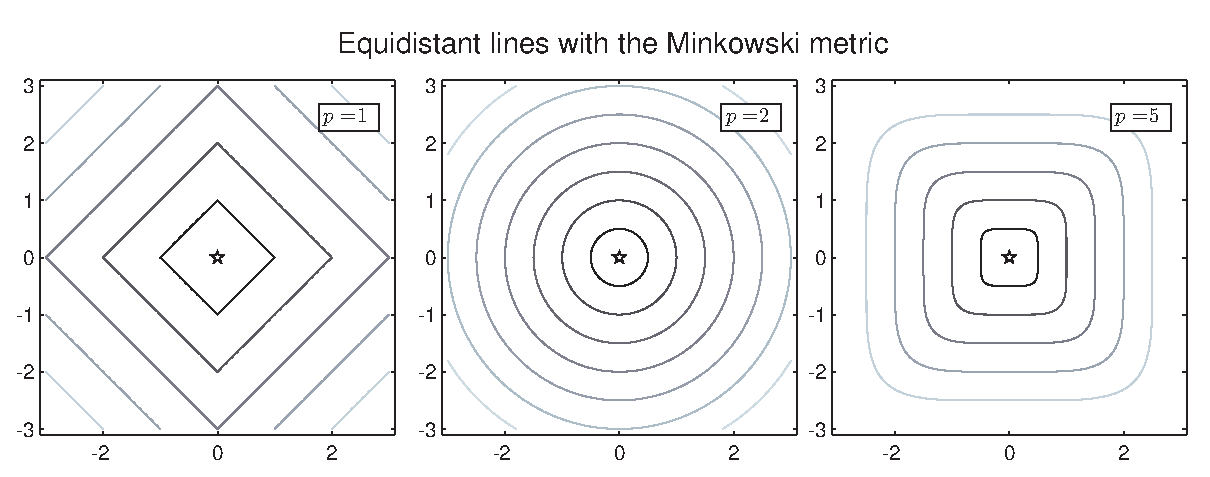
\includegraphics[width=\textwidth]{pics/minkowski_metrics.eps}%}
\caption[Equidistance lines using the Minkowski metric]{Visualization of the equidistance lines from the origin using the 
Minkowski metric with different values of $p$.}
\label{fig:Minkowski}
\end{figure}
\begin{equation}
\label{eq:minkowski}
 d^p(\v{x},\v{w}) = \left(\sum_{i=1}^N |x_i-w_i|^p\right)^\frac{1}{p}
\end{equation}
with $p=2$. 
Examples of the equidistance lines using the Minkowski metric and different values for $p$ are shown in Figure \ref{fig:Minkowski}. 
The classification takes places by a winner-takes-all scheme, i.e.\ a new data point $\v{x}$ is assigned to the class represented by 
the closest prototype:
\begin{equation}
\label{eq:nearest_prototype_classification}
 \v{x} \leftarrow c(\v{w}^i)\text{, with }\v{w}^i=\arg\underset{j}{\min}\ d(\v{x},\v{w}^j),
\end{equation}
braking ties arbitrary. The set of protoytpes and the metric is partitioning the input data space. 
Each prototype $\v{w}^i$ has a receptive field $R^i$\newnot{symbol:R^i}, which is a region in the feature space where $\v{w}^i$ 
is closer to the data than any other prototype:
\begin{equation}
\label{eq:Receptive_field_prototypes}
 R^i = \{ \v{x}\in \C{X}|\ d(\v{x},\v{w}^i)<d(\v{x},\v{w}^j), \forall i\neq j \} \enspace .
\end{equation}
Figure \ref{fig:NPC} shows two examples of nearest prototype classification on a three class problem using different distance measures. 
The Euclidean distance leads piecewise linear decision boundaries and receptive fields. 
For different values of $p$ in the Minkowski metric more general decision boundaries can be realized. 

The number of protoytpes is a hyper-parameter of the model and has to be optimized by means of a validation procedure.  
Too few prototypes may not represent the data structure sufficiently, which yields poor classification performance and 
too many prototypes may cause overfitting leading to poor generalization ability of the classifier. 
Many machine learning techniques have been proposed based on the nearest prototype classification scheme. 
Some of them used in the thesis will be addressed in the next sections. 

\begin{figure}[tpb]
\centering
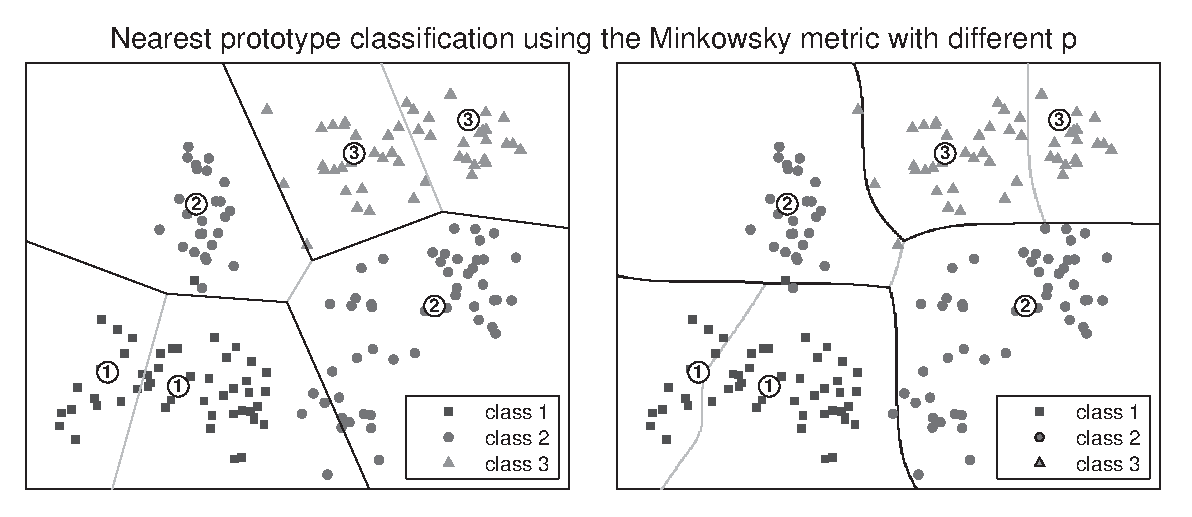
\includegraphics[width=\textwidth]{pics/NPC.eps}%}
\caption[Nearest prototype classification]{Visualization of the decision bounds of a nearest prototype classification scheme 
using different distances. The data is consisting of 3 classes and each class is represented by two prototypes. 
The Euclidean distance (left panel) shows piecewise linear boundaries where the gray lines denote the receptive fields of each prototype. 
In the right panel the Minkowski metric of order $p=5$ is used.% leading to nonlinear bounds.
}
\label{fig:NPC}
\end{figure}\index{Classification!Nearest prototype classification}